\section{Study Area}
To verify to performance of the developed method these criteria were used for selecting a study area:
\begin{enumerate*}[(i)]
	\item concerns an agricultural landscape,
	\item contains a variety of linear vegetation elements (straight, curves, corners, attached to non-linear elements), and
	\item contains non-linear vegetation elements.
\end{enumerate*}
These criteria ensure the both the classification of vegetation and delineation of linear elements can be properly trained and tested.

The chosen study area is located in an agricultural landscape in the middle of the Netherlands between Beesd in the west and Geldermalsen in the east (figure~\ref{fig:ResearchArea}). The area is about 1.6 km from east to west and 1.2 km from north to south, spanning an area of almost 2 million square meters. 
\begin{figure}
	\centering
	\fbox{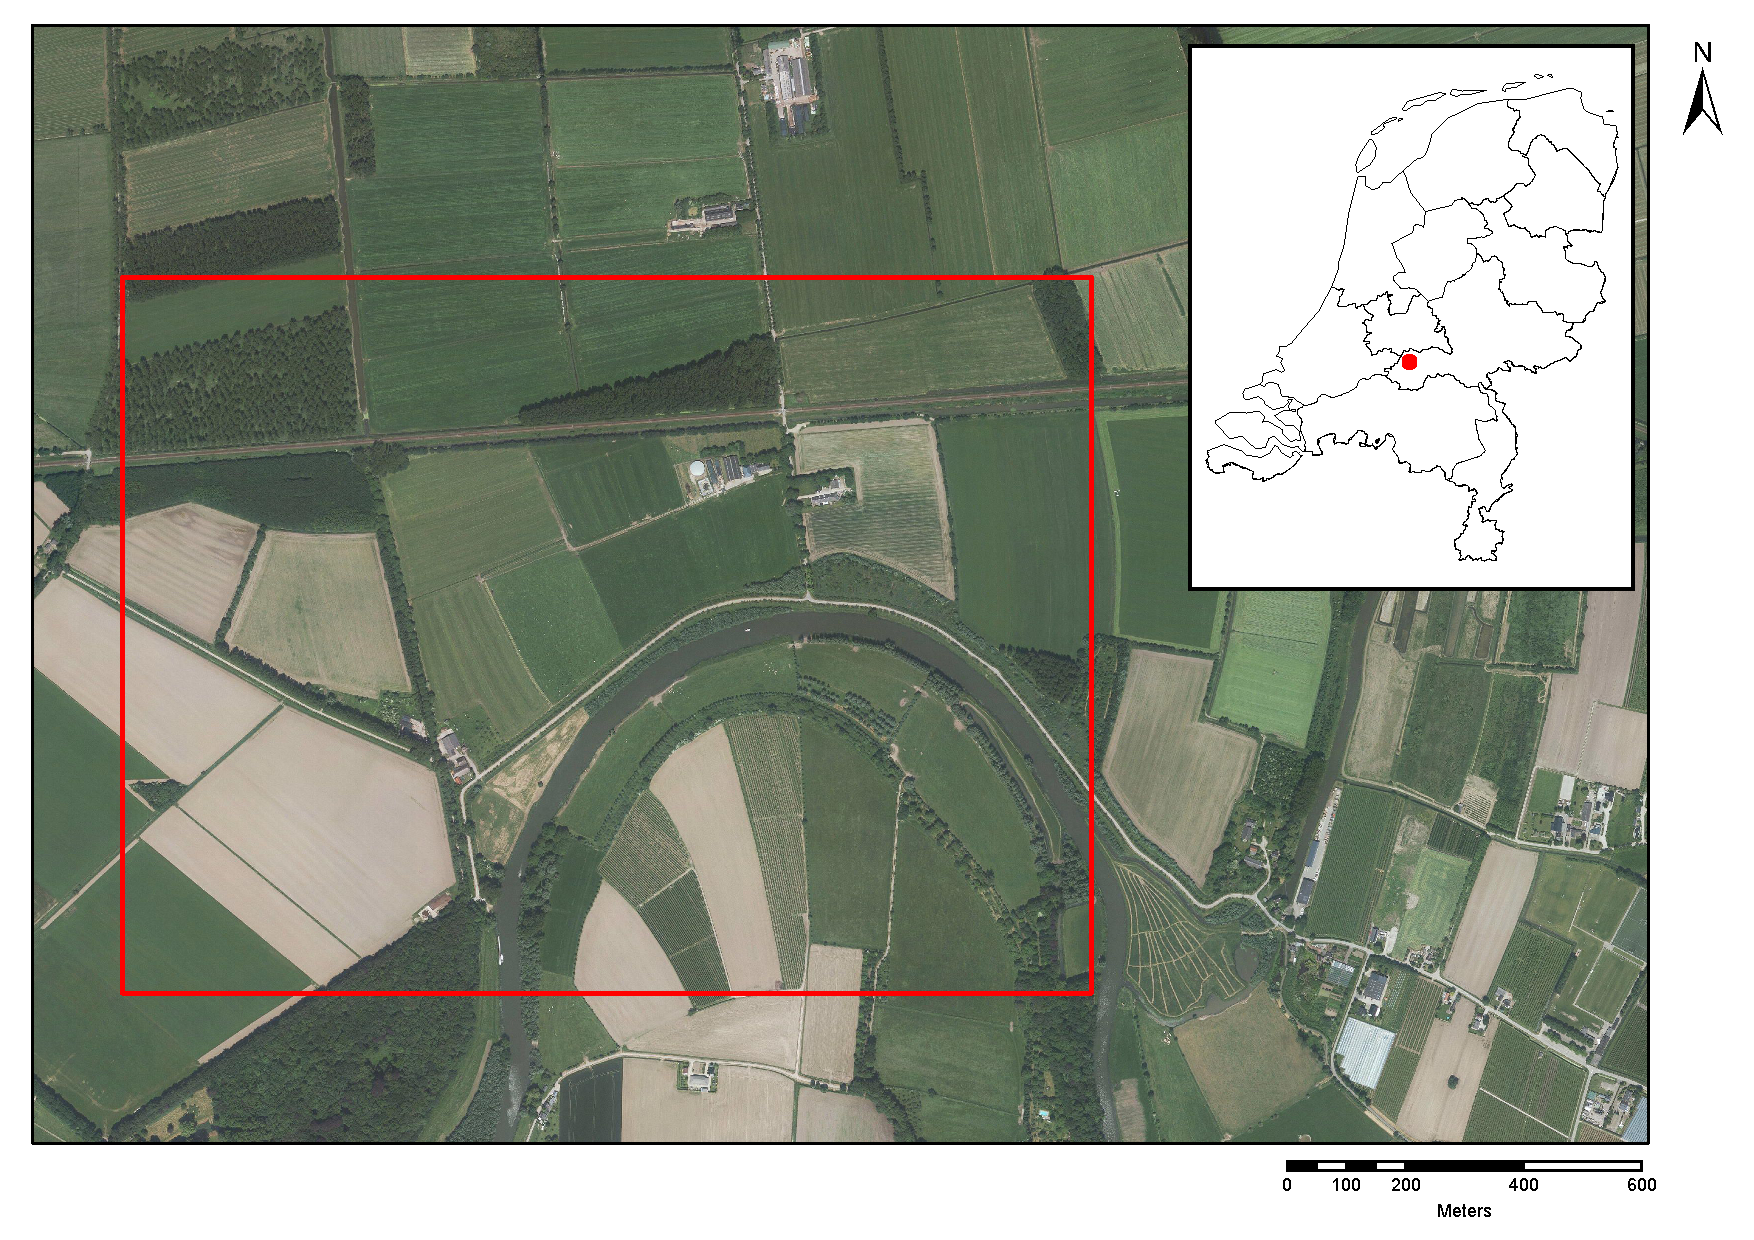
\includegraphics[scale=0.42]{./img/ResearchArea}}
	\caption{The study area.}
	\label{fig:ResearchArea}
\end{figure}